\chapter{Przegląd stanu wiedzy}\label{chap:teoria}
\section{Uczenie maszynowe}\label{machine_learning}
Mówi się, że program komputerowy uczy się z doświadczenia (\textit{experience}) E w związku z pewną klasą zadań (\textit{tasks}) T oraz miarą wydajności (\textit{performance measure}) P jeżeli jego osiągi w zadaniach w T, jak mierzone przez P, ulegają polepszeniu z doświadczeniem E. \cite{mitchell1997machine}
W przypadku pojedynczej konwolucyjnej sieci neuronowej (opisanej bliżej w \ref{sec:cnn}):
\begin{itemize}
	\item jako doświadczenie $E_{CN}$ możemy zdefiniować przetwarzanie obrazów wraz z ich etykietami klas
	\item zadaniem $T_{CN}$ nazwiemy klasyfikację obrazów
	\item miarą jakości $P_{CN}$ będzie stosunek liczby poprawnie zaklasyfikowanych zdjęć ze zbioru testowego do wielkości zbioru testowego
\end{itemize}
W przypadku algorytmu genetycznego (opisanego w \ref{sec:ag}) poszukującego optymalnej struktury sieci neurnowej:
\begin{itemize}
	\item doświadczeniem $E_{GA}$ będzie tworzenie i testowanie nowych sieci neruonowych
	\item zadanie $T_{GA}$ to poszukiwanie optymalnej w sensie $P_{CN}$ struktury (parametrów) sieci neuronowej
	\item miarą jakości $P_{GA}$ będzie miara jakośći najlepszego wygenerowanego przez algorytm osobnika
\end{itemize}
Zastosowanie jednego algorytmu z dziedziny uczenia maszynowego do poprawy procesu uczenia się innego algorytmu tej samej klasy ma ścisły związek z pojęciem metauczenia.
\section{Metauczenie}
\begin{enumerate}
	\item System metauczący się (\textit{A metalearning system}) musi zawierać podsystem uczący się, który przystosowuje się z doświadczeniem.
	\item Doświadczenie jest zdobywane poprzez wykorzystywanie metawiedzy wydobytej
	\begin{enumerate}[a)]
		\item z poprzedniego epizodu uczenia na pojedynczym zbiorze danych, i/lub
		\item z innych dziedzin lub problemów.
	\end{enumerate}
\end{enumerate}
Dodatkowo, często używanym pojęciem w metauczeniu jest pojęcie tendencyjnośći (\textit{bias}), które w tym kontekście odnosi się do zbioru założeń wpływająych na wybór hipotez opisujących dane. \cite{Lemke2015}
Hipoteza w tym kontekście oznacza funkcję predykcyjną (\textit{predictive function}) powstałą w wyniku zastosowania tradycyjnego uczenia (np. konwolucyjnej sieci neuronowej) pewnymi danymi, a wpływ na jej kształt mają ustalone założenia zaszyte w strukturze uczonego algorytmu. \cite[s.2]{Brazdil2009}
Autorzy w \cite{Brazdil2009} wyróżniają:
\begin{itemize}
	\item tendencyjność deklaratywną (\textit{declarative bias}) - specyfikuje ona reprezentację przestrzeni hipotez, np. przedstawianie hiptoez korzystając wyłącznie z sieci neuronowych
	\item tendencyjność proceduralną (\textit{procedural bias}) - wpływa na szeregowanie hipotez, np. preferowanie hipotez o krótszym czasie wykonania (\textit{runtime})
\end{itemize}
Zgodnie z tą teorią, w tradycyjnym uczeniu tendencyjność jest stała, podczas gdy metauczenie stara się ją dobierać dynamicznie. \cite{Lemke2015}
W kontekście projektowanego systemu automatycznie dobierającego parametry konwolucyjnej sieci neuronowej, spełnia ona założenia sprecyzowane w pierwszej części definicji, tj.
\begin{itemize}
	\item Istnieje uczący się podsystem (konwolucyjna sieć neurnowa)
	\item Struktura najlepszego osobnika ulega zmanie (przystosowuje się z doświadczeniem)
	\item Metawiedza jest wydobywana z poprzednich epizodów uczenia (jako wartość funkcji przystosowania konkretnej struktury)
\end{itemize}
W odniesieniu do tendencyjności deklaratywnej - przestrzeń poszukiwań (najlepszego algorytmu do klasyfikacji obrazów) została zawężona wyłącznie do konwolucyjnych sieci neruonowych, jednakże sieci o różnych strukturach będą produkować różne hipotezy.
Poszukiwanie najlepszego algorytmu do klasyfikacji obrazów na zbiorze CIFAR-10 nie jest tematem tej pracy - jest nią próba znalezienia optymalnej struktury dla konkretnego algorytmu.
W przypadku tak zawężonej przestrzeni poszukwiań dalej możemy preferować jedne generowane hipotezy od drugich, co można regulować odpowiednio modyfikując funkcję przystosowania, np. uwzględniając karę za komplikację uzyskanej struktury (np. wynikowa ilość aktywnych warstw konwolucyjnych).
\section{Uczenie z nadzorem}\label{supervised_learning}
Zadanie uczenia maszynowego nauczenia się funkcji wiążącej wejście z wyjściem na podstawie przykładowych par wejściowo-wyjściowych nazywamy uczeniem z nadzorem. \cite{russell2010artificial}
Polega ono na wywodzeniu funkcji z oznaczonych etykietami danych treningowych składających się ze zbioru przykładów treningowych. \cite{mohri2012foundations}
Przykładowy problem, który może zostać zaklasyfikowany do uczenia z nadzorem: posiadając historyczne dane miesięczne na temat ilości pożarów w danym mieście, przewidzieć ile pożarów wybuchnie w nadchodzącym miesiącu.
W tym wypadku czas (miesiąc) jest zmienną niezależną, a liczba pożarów zmienną zależną. Ustalenie związku pomiędzy tymi wielkościami (znalezienie modelu) jest zadaniem regresji, które jest jedną z podklas uczenia z nadzorem.
Drugą klasą takich problemów jest tzw. problem klasyfikacji, w którym, zamiast wyznaczać funkcję, której zbiór wartości jest (w przybliżeniu) ciągły, identyfikujemy odwzorowane, które pozowli nam nową, nieznaną daną zakwalifikować do dykretnego zbioru klas.
Popularnym przykładem jest uczenie systemu klasyfikowania wiadomości e-mail jako spam lub nie, gdy posiadamy zbiór treningowy w postaci już opisanych jako należące do odpowiedniej klasy wiadomośći.
Podczas gdy taki klasyfikator (filtr antyspamowy) przetwarza tekst, w przypadku niniejszej pracy magisterskiej mamy do czynienia z problemem klasyfikacji obrazów.
\section{Klasyfikacja obrazów}
Klasyfikacja obrazów jest zadaniem z klasy uczenia z nadzorem, w którym poszukujemy funkcji przypisującej obrazom odpowiednie etykiety z pewnego skończonego zbioru.
Jest to jeden z podstawowych problemów przetwarzania obrazów.
Co więcej, wiele pozornie różnych zadań (takich jak detekcja obiektów, segmentacja) można zredukować do problemu klasyfikacji obrazów.
Przykładowo, model klasyfikujący obrazy przetwarza zdjęcie pokazane poniżej na rys. \ref{fig:image_classification} i przypisuje prawdopodobieństwa do czterech kategorii, $\lbrace kot, pies, kapelusz, kubek \rbrace$.
Jak pokazano na rysunku, należy pamiętać, że zdjęcia dla komputera są niczym innym jak dużą trójwymiarową tablicą liczb.
W tym przypadku zdjęcie kota jest szerokie na 2048 pikseli, wysokie na 1536 pikseli i posiada 3 kanały koloru: czerwony, zielony i niebieski (z ang. w skrócie \textit{RGB}).
Tym samym zdjęcie składa się z $2048 \times 1536 \times 3 = 9437184$ liczb.

\begin{figure}[h!tb]
	 \centering
	 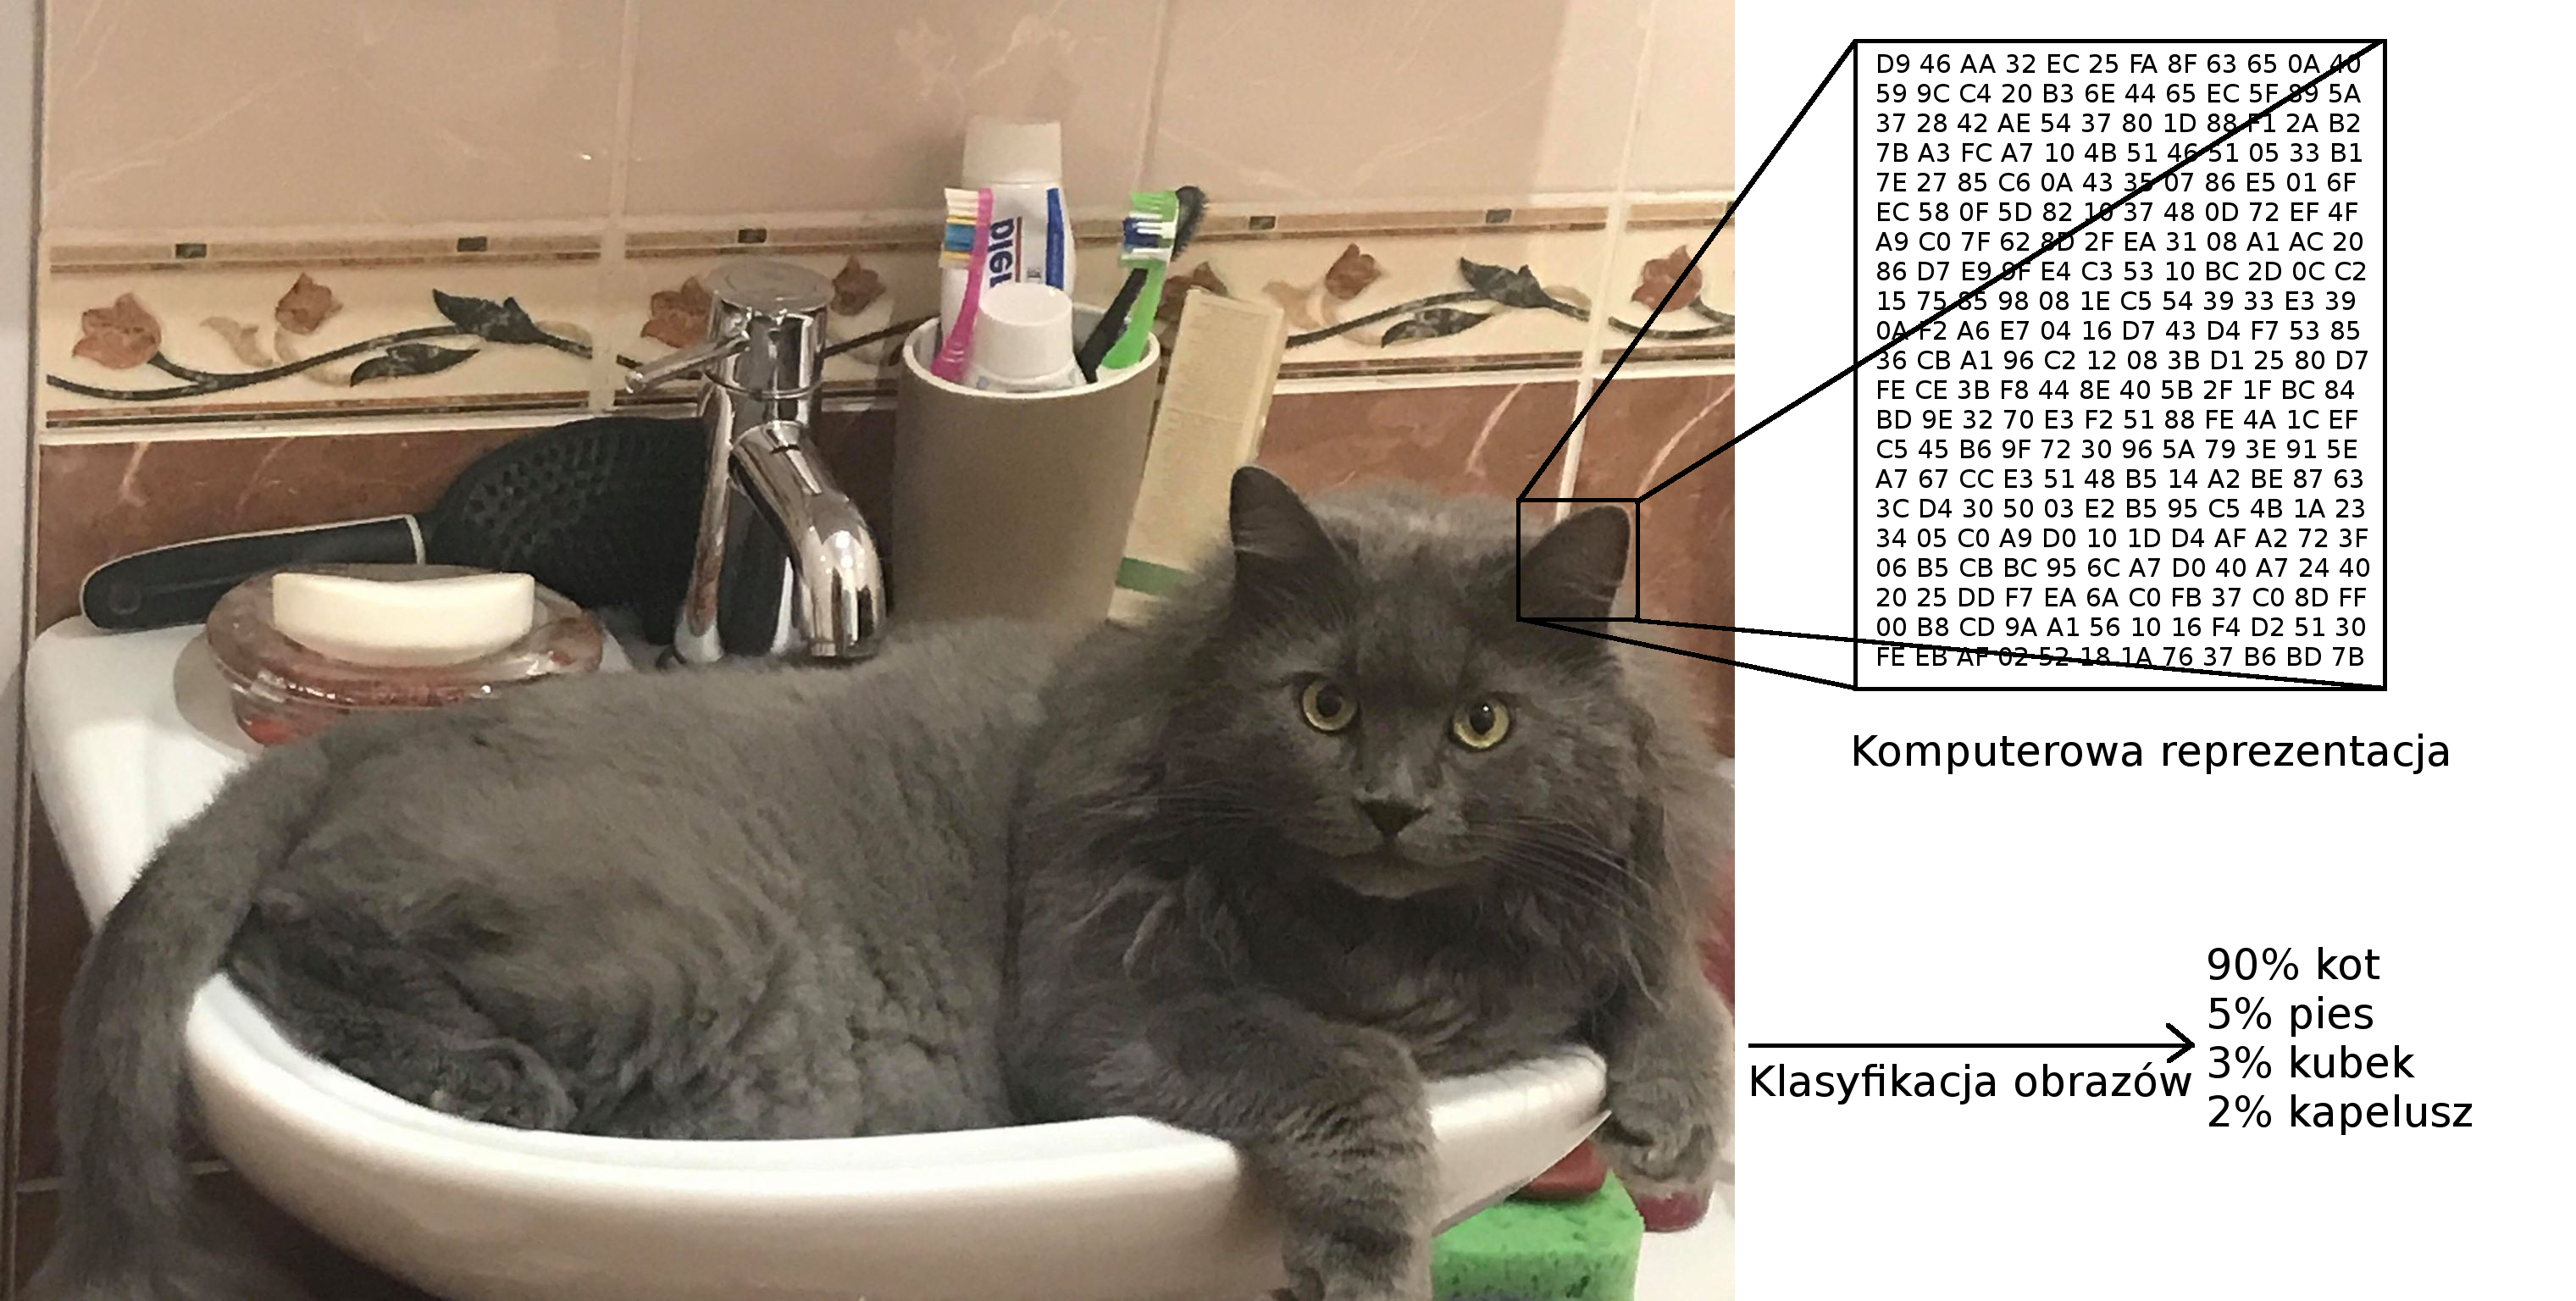
\includegraphics[width = 1.0\linewidth]{img/kot}
	 \caption{Komputerowa reprezentacja zdjęcia kota \\
              Źródło: praca własna na podstawie \cite{cs231n}}
	 \label{fig:image_classification}
\end{figure}

Zadanie klasyfikacji obrazów w tym przypadku polega na zredukowaniu tych prawie 10 milionów liczb do jednej etykiety, dla rys. \ref{fig:image_classification} będzie to ''$kot$''.
Dla człowieka rozpoznanie obiektu jest względnie proste. Z punktu widzenia algorytmu przetwarzania obrazów napotykamy kilka zasadniczych trudności, związanych z faktem, że komputer interpretuje obraz jako trójwymiarową macierz wartości jasności pikseli:
\begin{itemize}
	\item Zróżnicowanie perspektywy - ten sam obiekt może być różnie zorientowany względem kamery rejestrującej obraz
	\item Zróżnicowanie skali - obiekty jednej klasy (np. koty) często występują w różnych rozmiarach (nie tylko z punktu widzenia rozmiaru na zdjęciu, ale i w rzeczywistości)
	\item Deformacja - wiele klasyfikowanych obiektów nie jest bryłami sztywnymi i mogą być skrajnie zniekształcone
	\item Okluzja - zjawisko zasłonięcia obiektu przez inny obiekt, czasem jedynie niewielki fragment szukanego obiektu jest widoczny
	\item Warunki oświetleniowe - efekty różnego oświetlenia są bardzo wydatne na poziomie pikseli
	\item Nieład w tle - klasyfikowane obiekty mogą zlewać się z tłem, czyniąc ich identyfikację trudniejszą
	\item Zróżnicowanie wewnątrz klasy - niektóre klasy są bardzo ogólne (np. broń) i zawierają w sobie bardzo różnie wyglądające obiekty (np. miecz a karabin maszynowy).
\end{itemize}
Na rys.\ref{fig:classification_problems} przedstawiono ilustrację powyższych problemów.

\begin{figure}[h!tb]
	 \centering
	 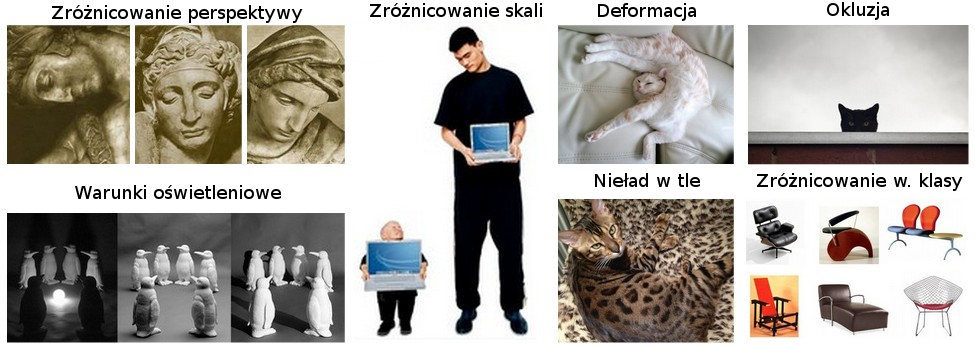
\includegraphics[width = 1.0\linewidth]{img/klas_problemy}
	 \caption{Problemy w klasyfikacji obrazów \\
              Źródło: praca własna na podstawie \cite{cs231n}}
	 \label{fig:classification_problems}
\end{figure}

Dobry model klasyfikujący obrazy powienien być niewrażliwy na dowolne kombinacje powyższych zakłóceń, jednocześnie pozostając wrażliwym na zróżnicowanie pomiędzy klasami.
Stworzenie algorytmu poprawnie klasyfikującego obrazy jest zadaniem nietrywialnym (w przeciwieństwie np. do ułożenia algorytmu sortującego liczby według zadanego porządku).
Jednym ze podejść, jakie można przyjąć do tego problemu, jest stworzenie algorytmu, który będzie się uczył na podstawie dużej ilości oznaczonych etykietami danych, czyli wspomniane wcześniej uczenie maszynowe (\ref{machine_learning}) i uczenie z nadzorem (\ref{supervised_learning}).
Takie rozwiązanie problemu nazywane jest również podejściem opartym na danych (\textit{data-driven approach}).
\cite{cs231n}


\section{CIFAR-10}
Przykładem zbioru danych służącego do uczenia i oceny algorytmów uczenia maszynowego w dziedzinie klasyfikacji obrazów jest zbiór CIFAR-10.
Zbiór danych CIFAR-10 składa się z 60000 kolorowych obrazków o wymiarach 32x32 pogrupowanych w 10 klas, po 6000 obrazków w każdej. Zbiór trenigowy składa się z 50000 obrazków, a testowy z 10000.

Dane zorganizowane są w pięć partii trenigowych i jedną testową, po 10000 obrazków każda. Partia testowa zawiera dokładnie po 1000 losowo wybranych obrazków z każdej klasy. Partie treningowe zawierają pozostałe obrazki w losowej kolejności, w związku z czym niektóre partie mogą zawierać więcej obrazków z jednej klasy niż pozostałych. Łącznie zawierają po 5000 obrazków z każdej klasy.

Poniżej, na rysunku \ref{fig:sample_data} przedstawiono wszystkie klasy wraz z 10 losowymi obrazkami dla każdej z nich.
\begin{figure}[h!tb]
	 \centering
	 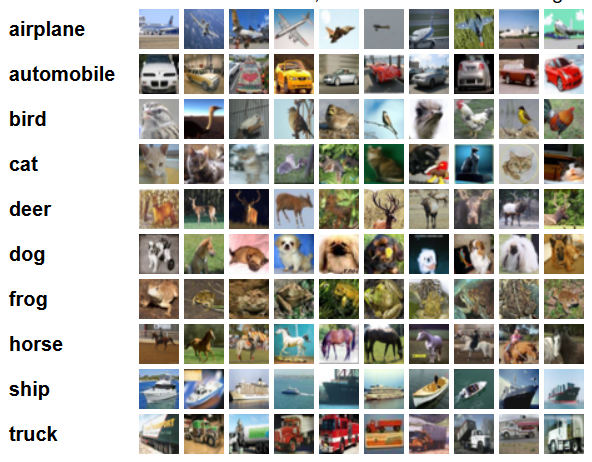
\includegraphics[width = 1.0\linewidth]{img/sample_images}
	 \caption{Przykładowe obrazki ze zbioru CIFAR-10 \\
              Źródło: https://www.cs.toronto.edu/\textasciitilde kriz/cifar.html}
	 \label{fig:sample_data}
\end{figure}

Każda z klas wyklucza się wzajemnie. Klasy ''samochód'' (\textit{automobile}) i ''ciężarówka'' (\textit{truck}) nie posiadają części wspólnej. ''Samochód'' zawiera sedany, SUVy i inne tego typu samochody. ''Ciężarówka'' zaiwera tylko duże ciężarówki. Żadna z nich nie zawiera pojazdów typu pickup.

Poniżej opisano organizację tego zbioru danych w wersji dla języka Python.

Archiwum zawiera pliki data\_batch1, data\_batch2 data\_batch5, jak również test\_batch. Każdy z tych plików jest poddaną serializacji wersją obiektu Pythonowego wytworzonego za pomocą cPickle. Poniżej, na listingu \ref{lst:read_data} przedstawiono procedurę odczytującą te pliki i zwracającą słownik dla Pythona w wersji 2:

\begin{lstlisting}[caption={Procedura ładowania zbioru danych},label={lst:read_data},language=Python,captionpos=b,frame=single]
def unpickle(file):
    import cPickle
    with open(file, 'rb') as fo:
        dict = cPickle.load(fo)
    return dict
\end{lstlisting}

    Załadowane w ten sposób, każdy z plików z partiami zawiera następujące elementy:
\begin{itemize}
\item \textit{data} - macierz \textit{numpy} typu \textit{uint8} o wymiarach 10000x3072. Każdy rząd macierzy przechowuje kolorowy obrazek o wymiarach 32x32. Pierwsze 1024 pozycji zawiera wartości pikseli dla kanału czerwononego, kolejne 1024 dla zielonego, a ostatnie dla niebieskiego. Zdjęcia przechowywane są rzędami w kolejności od góry do dołu, tj. pierwsze 32 elementy macierzy opisują wartości kanału czerwonogo dla pierwszego rzędu pikseli obrazka.
\item \textit{labels} - lista 10000 liczb w przedziale 0-9. Liczba pod indeksem i oznacza etykietę z klasą dla i-tego obrazka w macierzy data.
\end{itemize}

Zbiór danych zawiera również plik batches.meta, który również zawiera obiekt typu słownik dla języka Python. Zawiera on następujące elementy:
\begin{itemize}
\item \textit{label\_names} - 10 elementowa lista która nadaje czytelne dla człowieka nazwy liczbowym etykietom w liście \textit{labels} opisanej powyżej. Na przykład, label\_names[0] == ''airplane'', label\_names[1] == ''automobile'', itd. \cite{Krizhevsky09learningmultiple}
\end{itemize}

Wśród kilku podejść, które mogą nam posłużyć do rozwiązania tego problemu, wyróżnić możemy algorytm k najbliższych sąsiadów (\textit{k - Nearest Neighbour Classifier}), klasyfikatory liniowe, sieci neuronowe.

\section{K najbliższych sąsiadów}\label{sec:knear}

Dla zbioru CIFAR-10 mamy $50000$ obrazków oznaczonych etykietami i $10000$ obrazów, które chcemy zaklasyfikować.
Każdy obrazek o wymiarach $32 \times 32 \times 3$ możemy przedstawić jako wektor o wymiarach $3072 \times 1$.
Oznacza to, że każdy z nich możemy interpretować jako punkt w przestrzeni $3072$-wymiarowej.
Najprotszym sposobem w jaki możemy klasyfikować nowe dane jest badanie ich położenia w owej przestrzeni.
Zakładając, że obrazki jednej klasy będą grupować się w klastry, każdy kolejny punkt znajdujący się blisko chmury punktów reprezentującej daną klasę z wysokim prawdopoboieństwem również będzie przynależał do tej klasy.
Przykładowo, rozważmy sytuację jak na rys. \ref{fig:knearest} dla klasyfikacji dwuwymiarowych punktów. Punkt albo przynależy do klasy 'niebieski okrąg', albo 'czerwony krzyżyk'. Rozważamy punkt, który oznaczony jest zielonym krzyżykiem.

\begin{figure}[h!tb]
	 \centering
	 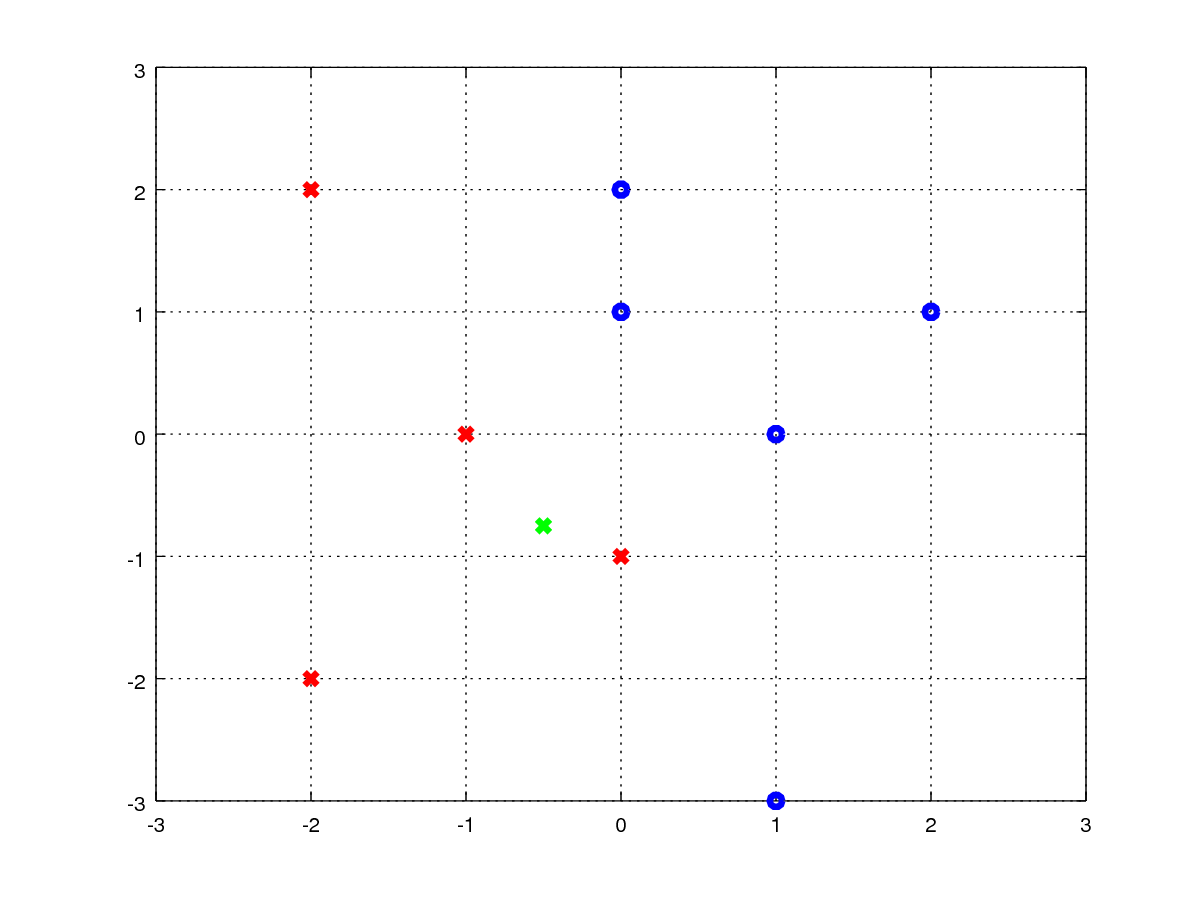
\includegraphics[width = 1.0\linewidth]{img/knear}
	 \caption{Ilustracja działania algorytmu k najbliższych sąsiadów w dwóch wymiarach \\
              Źródło: praca własna}
	 \label{fig:knearest}
\end{figure}

Dla najprostszego przypadku $k=1$ badamy odległości (w tym przypadku użwyając normy $l^2$) pomiędzy interesującym nas punktem a wszystkimi danymi ze zbioru treningowego i przyjmujemy, że badany punkt będzie przynależał do tej samej klasy, do której przynależy jej najbliższy sąsiad.
W przypadku rys. \ref{fig:knearest} badany zielony punkt znajduje się najbliżej czerwonego krzyżyka w punkcie $(0,-1)$, zatem przypisujemy go do tej samej klasy.
Dla większych wartości k rozważamy więcej najbliższych sąsiadów i przypisujemy rozważany punkt do tej klasy, do której należy większość najbliższych punktów.

Podejście to, mimo iż intuicyjne i proste w implementacji, nie rozwiązuje dobrze problemu klasyfikacji, osiągając skuteczność $39.6\%$ dla $k = 1$ dla zbioru CIFAR-10.
Jest to lepiej niż losowe przydielanie do klas (które dla 10 klas ma skuteczność $10\%$), ale wciąż dalekie od skuteczności człowieka.

Jednym z problemów podejścia k najbliższych sąsiadów jest kosztowne testowanie nowych punktów.
Dla każdego nowego punktu wymaga ono policzenia odległości od 50000 punktów w przestrzeni 3072-wymiarowej oraz posortowania wg. obliczonej odległości, co jest dość kosztowną operacją.

Kolejnym problemem w przypadku przetwarzania obrazów jest klasyfikowanie wyłącznie na podstawie dominujących w obrazie wartości kolorów.
Na przykład, zarówno w przypadku klasy ''samolot'' jak i w przypadku klasy ''statek'' często występującym w tle kolorem będzie niebieski, gdyż niebieskie jest zarówno niebo i woda.
Tak duże podobieństwo może prowadzić do błędnej klasyfikacji w przypadku tych dwóch klas. \cite{cs231n}

\section{Klasyfikator liniowy}

Innym podejściem, jakie można przyjąć do klasyfikacji obrazów, jest stworzenie liniowego odwzorowania pomiędzy pikselową reprezentacją obrazu a stopniem przynależności danego obrazu do poszczególnych klas.
Oznaczając dane treningowe przez $x_i \in R^D$, każde powiązane z etykietą $y_i$.
W tym przypadku $i = 1 ... N$ i $y_i \in 1 ... K$, tj. zbiór uczący składa się z $N$ przykładów (każdy D-wymiarowy) i K rozróżnialnych kategorii.
Przykładowo, dla zbioru CIFAR-10 zbiór treningowy ma rozmiar $N = 50000$, każdy po $32 \times 32 \times 3 = 3072$ pikseli i $K = 10$, poniważ rozróżniamy pomiędzy 10 klasami (pies, kot, samochód itd.).
Zdefiniujemy funkcję oceny (\textit{score function}) $f : R^D \mapsto R^K$, która odwzorowuje wartości pikseli do oceny przynależności do danej klasy.
Zatem liniowy klasyfikator zdefiniować jako następujące liniowe odwzorowanie:
\begin{equation}\label{eqn:lc}
f(x_i,W,b) = Wx_i + b
\end{equation}
We wzorze \ref{eqn:lc} zakładamy, że obrazek $x_i$ zawiera wszystkie wartości swoich pikseli w wektorze o wymiarach $[D \times 1]$.
Macierz $W$ (o wymiarach $[K \times D$]) oraz wektor $b$ (o wymiarach [$K \times 1$]) są parametrami funkcji.
W zbiorze CIFAR-10 $x_i$ zawiera wszystkie piksele $i$-tego obrazka spłaszczone do jednej [$3072 \times 1$] kolumny, $W$ ma wymiar [$10 \times 3072$] a $b$ [$10 \times 1$], zatem 3072 liczby są wejściem dla funkcji, a wyjść jest 10 (oceny klas).
Parametry wewnątrz $W$ nazywane są również wagami, a wektor $b$ nazywany jest wektorem przesunięcia (\textit{bias vector}), ponieważ ma wpływ na wyjściowe ocenu bez wchodzenia w interakcję z danymi $x_i$. \cite{cs231n}

Jak już wspominano, obrazki mogą być rozumiane jako punkty w 3072 wymiarowej przestrzeni.
Pojedynczy liniowy klasyfikator możemy interpretować jako hiperpłaszczyznę separującą punkty w tej przestrzeni.
Możemy wyobrazić sobie ściśnięcie wszystkich punktów do dwóch wymiarów jak na rys. \ref{fig:cartoon_class}, wtedy hiperpłaszczyny sprowadzają się do prostych.

\begin{figure}[h!tb]
	 \centering
	 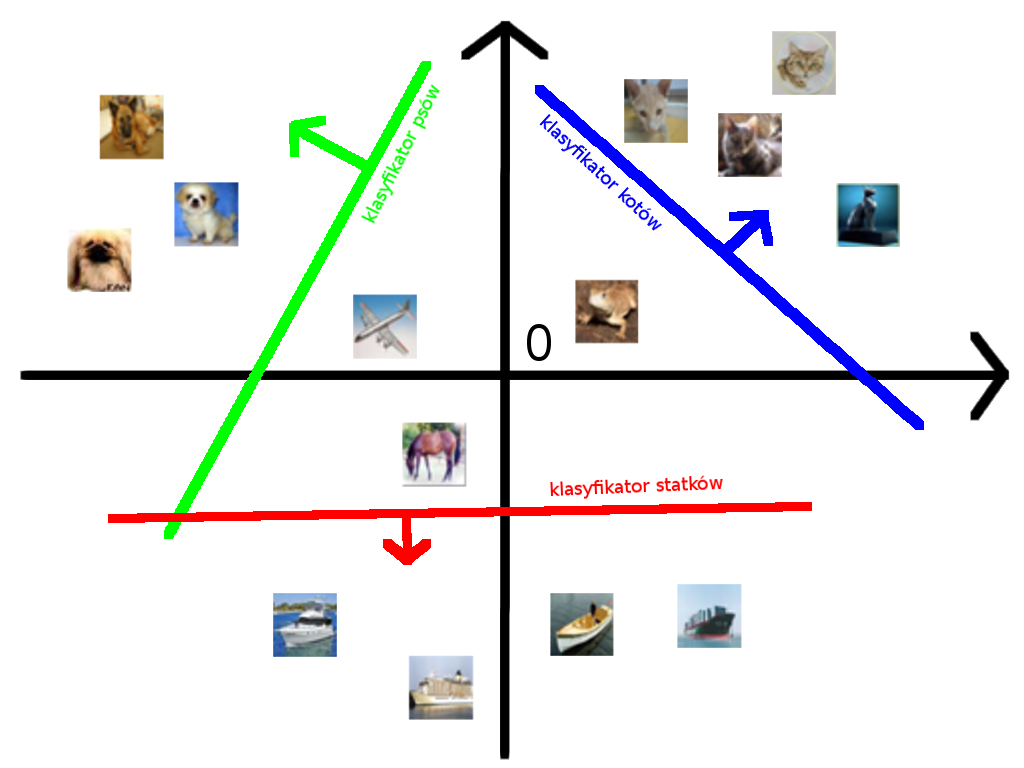
\includegraphics[width = 0.75\linewidth]{img/klas_cartoon}
	 \caption{Schematyczna wizualizacja działania klasyfikatorów liniowych \\
              Źródło: praca własna na podstawie \cite{cs231n}}
	 \label{fig:cartoon_class}
\end{figure}

Przy klasyfikatorze liniowym warto zauważyć kilka faktów:
\begin{itemize}
	\item Pojedyncze mnożenie macierzowe $Wx_i$ w efekcie wyznacza oceny dla 10 różnnych klasyfikatorów jednocześnie (jeden na klasę), gdzie każdy klasyfikator to rząd macierzy W i jednej prostej separującej na rys. \ref{fig:cartoon_class}
	\item Dane wejściowe $(x_i,y_i)$ są ustalone, a kontrolujemy parametry $W,b$. Naszym celem będzie ustawienie tych parametrów w taki sposób, by wynikowe oceny zgadzały się z prawdziwymi przynależnościami do klas na całym zbiorze treningowym.
	\item Zaletą tego podejścia jest możliwość odrzucenia (nie przechowywania w pamięci) zbioru treningowego po nauczeniu się parametrów $W,b$. Dzieje się tak, ponieważ nowe punkty do klasyfikacji klasyfikujemy przy pomocy ocen uzyskanych z już nauczonej funkcji.
	\item Klasyfikowanie obrazów testowych sprowadza się do pojedynczego mnożenia macierzowego i dodawania, które jest szybsze od porównywania do wszystkich obrazków ze zbioru treningowego (jak w \ref{sec:knear}).
\end{itemize}

Przykład mapowania wartości pikseli do oceny przynależności do klas przedstawiono na rys. \ref{fig:lin_class}
\begin{figure}[h!tb]
	 \centering
	 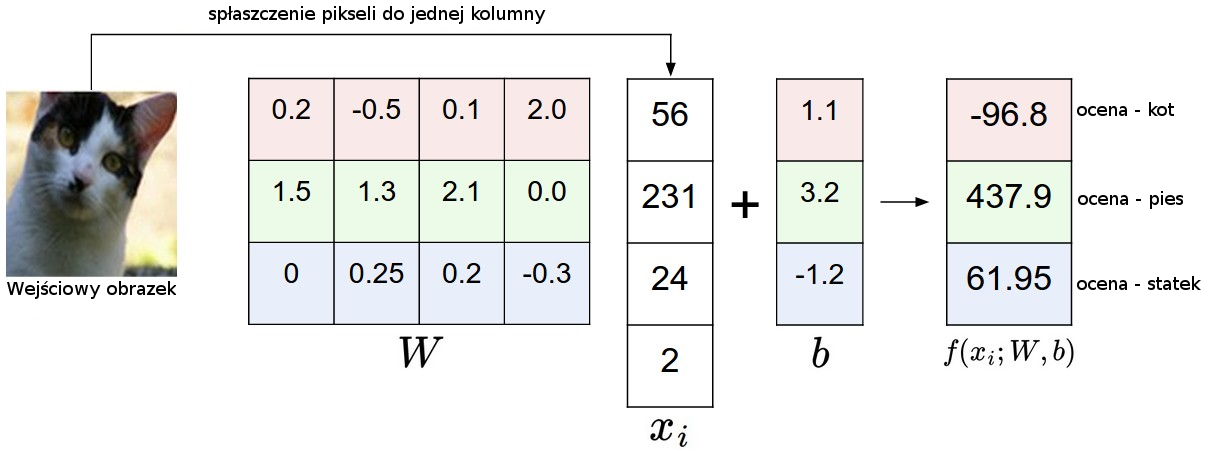
\includegraphics[width = 1.0\linewidth]{img/lin_klas}
	 \caption{Mapowanie 4 monochromatycznych pikseli do 3 klas \\
              Źródło: praca własna na podstawie \cite{cs231n}}
	 \label{fig:lin_class}
\end{figure}

Jak widać na rys. \ref{fig:lin_class}, wagi w macierzy W nie są dobrze dobrane, gdyż klasyfikator przypisuje najwyższą ocenę klasie pies, podczas gdy w istocie na obrazku znajduje się kot.
Uczenie liniowego klasyfikatora będzie polegać na takim doborze wag, by błędy klasyfikacji zachodziły jak najrzadziej.
W tym celu zdefinujemy funkcję kosztów (\textit{loss function}), która będzie miarą tego jak dobrze działa dany klasyfikator.\cite{cs231n}

Funkcję kosztów dla całego zbioru danych definuje wzór \ref{eqn:total_loss}.
\begin{equation}\label{eqn:total_loss}
L =  \underbrace{ \frac{1}{N} \sum_i L_i }_\text{składowa danych} + \underbrace{ \lambda R(W) }_\text{składowa regularyzacji} \\\\
\end{equation}
gdzie $\lambda$ jest parametrem kontrolującym oddziaływanie regularyzacji przy uczeniu, $L_i$ wartością funkcji kosztu dla pojedynczego obrazka przy ustalonych wagach W (wzór \ref{eqn:single_loss_svm} lub \ref{eqn:single_loss_softmax}).
Składowa regularyzacji penalizuje duże wagi w macierzy $W$ i w tym przypadku będzie definiowana jako norma $l^2$ dla tej macierzy, zgodnie ze wzorem \ref{eqn:regularization}.

\begin{equation}\label{eqn:regularization}
R(W) = \sum_k\sum_l W_{k,l}^2
\end{equation}

Wprowadzenie tej składowej do funkcji kosztu pozwala uniknąć niejednoznaczności rozwiązania, gdzie dowolna macierz $W$ przeskalowana o współczynnik $\alpha \in R^+$ jest równie dobrym rozwiązaniem.
W ten sposób prefeorwane będą rozwiązania o o mniejszych wartościach współczynników.
Co więcej, okazuje się, że przy takim podejściu uzyskujemy lepiej generalizujące i bardziej odporne na nadmierne dopasowanie (\textit{overfitting}) klasyfikatory.
Wynika to z faktu, że żaden z wejściowych wymiarów nie może mieć dużego wpływu na końcowy wynik.
Dla przykładu, dla wektora danych $x = [1,1,1,1]$ i dwóch wektorów wagowych $w_1 = [1,0,0,0]$ i $w_2 = [0.25,0.25,0.25,0.25]$ wynik mnożenia (wartość funkcji oceny) $w_1^Tx = w_2^Tx = 1$.
Jednakże wprowadzenie kary $l^2$ do funkcji kosztu powoduje, że preferowany będzie wektor $w_2$, gdyż $||w_2|| < ||w_1||$, a naszym celem jest minimalizacja funkcji kosztów.
Widać zatem, że preferowane będą wektory wagowe o bardziej rozłożonych współczynnikach.

Składowa danych ze wzoru \ref{eqn:total_loss} jest funkcją kosztu dla pojedynczego obrazka uśrednioną po wszystkich danych treningowych.
Dla $i$-tego punktu treningowego możemy zdefinować wiele różnych funkcji kosztu.
Dla klasyfikatora typu wieloklasowa maszyna wektorów nośnych (\textit{Multiclass SVM}) będzie to koszt ''zawiasowy'' (\textit{hinge loss}, wzór \ref{eqn:single_loss_svm}), natomiast dla klasyfikatora typu \textit{Softmax} koszt entropii krzyżowej (\textit{cross-entropy loss}, przedstawiony na wzorze \ref{eqn:single_loss_softmax}).
\begin{equation}\label{eqn:single_loss_svm}
L_i = \sum_{j\neq y_i} \max(0, s_j - s_{y_i} + \Delta)
\end{equation}
gdzie $s_j = f(x_i, W)_j$ to $j$-ty element wektora ocen klas, $s_{y_i}$ jest oceną uzyskaną przez prawdziwą klasę, a $\Delta$ jest marigniesem, który chcemy utrzymać pomiędzy wartością oceny klasy prawdziwej a wartościami ocen klas niepoprawnych.

\begin{equation}\label{eqn:single_loss_softmax}
L_i = -\log\left(\frac{e^{s_{y_i}}}{ \sum_j e^{s_j} }\right) \hspace{0.5in} \text{lub równoważnie} \hspace{0.5in} L_i = -s_{y_i} + \log\sum_j e^{s_j}
\end{equation}
gdzie $s_j$ jak wyżej oznacza $j$-ty element wektora ocen klas $s$, tutaj interpretowany jako nieznormalizowany logarytm prawdopodobieństwa przynależności do danej klasy.

Możemy teraz znaleźć taką macierz wagową $W$, która minimalizuje wartość przyjętej funkcji kosztu, tym samym maksymalizując poprawność działania klasyfikatora.
Jest to problem optymalizacji, który rozwiązujemy najczęściej przy pomocy gradientowych metod optymalizacji, np. metody najszybszego spadku. \cite{cs231n}

Powodem, dla którego tyle miejsca poświęcono liniowemu klasyfikatorowi i pojęciami z nim związanymi jest fakt, że wszystkie te pojęcia mają również zastosowanie przy sieciach neuronowych.

\section{Sieci Neruonowe}\label{sec:nn}

\begin{figure}[h!tb]
	 \centering
	 \includegraphics[width = 1.0\linewidth]{img/neuron}
	 \caption{Pojedynczy 3-wejściowy neuron \\
              Źródło: praca własna na podstawie \cite{cs231n,zuradabarskijedruch1996}}
	 \label{fig:neuron}
\end{figure}

Zarówno zwierzęta, jak i ludzie lepiej radzą sobie z rozpoznawaniem obrazów niż współczesne komputery.
Sieci neuronowe dlatego wzbudzają zainteresowanie, że możemy za ich pomocą częściowo naśladować ludzki mózg.
Informacja w takich sieciach przetwarzana jest przez dużą ilość węzłów obliczeniowych oraz połączeń między nimi.
Skoordynowane jednoski jednocześnie dokonują przetwarzania wszystkich lub większości sygnałów i danych wejściowych.
Działanie sztucznych sieci neuronowych możemy porównać do rozproszonych systemów obliczeniowych.
Elementarną jednostkę wykonującą obliczenia w takiej sieci nazywamy neuronem.
Pojedynczy neuron dokonuje sumowania i nieliniowego przetwarzania sygnałów.
Nierzadko możemy je przyrównać do elementów działających progowo, aktywujących się w momencie przekroczenia pewnego zadanego progu przez sumę sygnałów na wejściu.
Często neurony organizowane są w regularne struktury, zwykle możemy w owych strukturach wyróżnić poszczególne warstwy.
Możliwe jest występowanie połączeń zwrotnych pomiędzy neuronami tej samej warstwy lub z różnych warstw.
Każde połączenie pomiędzy neuronami charakteryzowane jest przez siłę jego oddziaływania zwaną również wagą. \cite{zuradabarskijedruch1996}

Schematycznie pojedynczy neuron możemy przedstawić jak na rys. \ref{fig:neuron}

Architektura sieci jest tym co odróżnia konkretne sieci od siebie.
Na przykład sieci nie posiadające połączeń zwrotnych reagują na pobudzenie w sposób natychmiastowy i te własnie sieci będą omawiane w dalszej części pracy.
Natomiast sieci, które posiadają połączenia zwrotne, ustalają swoją odpowiedź dopiero po pewnym czasie, mają zatem swoją dynamikę określające ich zachowanie w czasie. \cite{zuradabarskijedruch1996}



\section{Konwolucyjne sieci neuronowe}\label{sec:cnn}

Konwolucyjne sieci neuronowe (\textit{Convolutional Neural Networks}) są podobne do opisanych w \ref{sec:nn} sieci neuronowych.
Tworzone są z neuronów, które posiadają swoje wagi, które zmieniają się w wyniku procesu uczenia.
Każdy z neuronów otrzymuje sygnały na wejściu, dokonuje ich sumowania, a następnie może dokonać nieliniowego odwzorowania.
Cała sieć wyraża pojedynczą, różniczkowalną funkcję odwzorowującą wartości jasności pikseli do zbioru klas.
Sieci te projektowane są z założeniem, że będą przetwarzały obrazy, stąd ich specyficzna architektura, która zostanie opisana poniżej.

Motywacją stojącą za poszukiwaniem innych architektur sieci neuronowych była bardzo szybko narastająca ilość wag do uczenia w przypadku przetwarzania obrazów za pomocą w pełni połączonych sieci neuronowych.
Biorąc dla przykładu CIFAR-10 i obrazki o wymiarach $ 32 \times 32 \times 3$ (wysokość, szerokość, 3 kanały kolorów), pojedynczy neuron znajdujący się zaraz za warstwą wejściową posiadałby 3072 + 1 wejście od stałej wartości (\textit{bias}) wag do nauczenia.
Dla tak małych obrazków liczba ta nie wydaje się być problematyczna, jednak podając na wejście obraz o wymiarach $1024 \times 768 \times 3 = 2359296$ widzimy, że już pojedynczy neuron zaczyna zajmować bardzo dużo pamięci.
Zakładając, że każda waga przechowywana jest jako liczba zmiennoprzecinkowa o podwójnej precyzji i przechowoywana w 8 bajtach, uzyskujemy $18874368$ B $= 18$MB na jeden neuron.
Tak duża liczba parametrów jest nadmiarowa i może prowadzić do nadmiernego dopasowania.

Konwolucyjne sieci neuronowe wykorzystują fakt, że danymi podawanymi na ich wejście są obrazy i nakładają ograniczenia na architekturę w bardziej rozsądny sposób.
W szególności, w przeciwieństwie do tradycyjnej sieci neuronowej, warstwy sieci konwolucyjnej posiadają neurony zorganizowane w 3 wymiarach: wysokości, szerokości i głębokośći (rozumianej jako trzeci wymiar wejścia, nie jako głębkość w sensie liczby warstw w sieci).
W sieciach neruonowych każda warstwa przekształca trójwymiarowe wejście na trójwymiarowe wyjście przez różniczkowalną funkcję, która może lecz nie musi posiadać parametry.

W sieciach konwolucyjnych wyróżnia się kilka podstawowych rodzajów warstw, które następnie składa się w całą sieć.
Trzy podstawowe typy to:
\begin{itemize}
	\item warstwa konwolucyjna lub splotowa - oblicza wyjścia neuronów połączynych z lokalnymi fragmentami wejścia, wyznaczając iloczyn skalarny pomiędzy swoimi wagami a małym obszarem wejścia, do którego są połączone.
	\item warstwa agregująca - dokonuje operacji podpróbkowania wzdłuż wysokośi i szerokośći wejścia, zmniejszając wymiar danych na swoim wyjściu
	\item warstwa w pełni połączona - tak jak w klasycznych sieciach neuronowych, każdy neuron jest połączony z każdą jednostką wejścia
\end{itemize}

Przyjmować będziemy również, że warstwa aktywacji liniowej (\textit{ReLU, Rectified Linear Unit}) jest ''zaszyta'' wewnątrz warstwy konwolucyjnej, na jej wyściu,
Warstwa ta realizuje funkcję $max(0, x)$ w odniesieniu do każdego elementu na swoim wejściu. \cite{cs231n}

\section{Algorytm geneteyczny}\label{sec:ag}

Algorytm genetyczny jest kolejnym opisywanym narzędziem sztucnej inteligencji, które powstało dzięki obsrerwacji natury i jej sposóbów działania.

Działanie algorytmu genetycznego można schematycznie przedstawić jak na rysunku \ref{fig:gen_schemat}

\begin{figure}[h!tb]
	 \centering
	 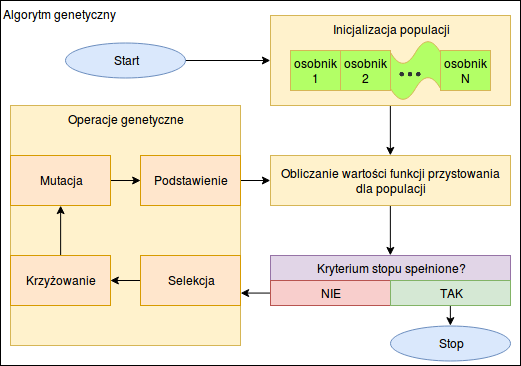
\includegraphics[width = 1.0\linewidth]{img/genetyczny_schemat}
	 \caption{Schemat działania algorytmu genetycznego \\
              Źródło: praca własna}
	 \label{fig:gen_schemat}
\end{figure}
